% Created 2021-02-26 Fri 10:36
% Intended LaTeX compiler: pdflatex
\documentclass[11pt]{article}
\usepackage[utf8]{inputenc}
\usepackage[T1]{fontenc}
\usepackage{graphicx}
\usepackage{grffile}
\usepackage{longtable}
\usepackage{wrapfig}
\usepackage{rotating}
\usepackage[normalem]{ulem}
\usepackage{amsmath}
\usepackage{textcomp}
\usepackage{amssymb}
\usepackage{capt-of}
\usepackage{hyperref}
\usepackage[margin=2cm]{geometry}
\author{Patryk Kaniewski}
\date{\today}
\title{}
\hypersetup{
 pdfauthor={Patryk Kaniewski},
 pdftitle={},
 pdfkeywords={},
 pdfsubject={},
 pdfcreator={Emacs 27.1 (Org mode 9.3)}, 
 pdflang={English}}
\begin{document}

\tableofcontents \clearpageOP source: \url{https://www.youtube.com/playlist?list=PLrhzvIcii6GNjpARdnO4ueTUAVR9eMBpc}
\section{SOLID}
\label{sec:org59768d4}
\subsection{single responsibility}
\label{sec:org6a0266b}
Klasa powinna mieć tylko jedną odpowiedzialność (nigdy nie powinien istnieć więcej niż jeden powód do modyfikacji klasy).
\subsection{open-closed principle}
\label{sec:org74bee9b}
Klasy (encje) powinny być otwarte na rozszerzenia i zamknięte na modyfikacje.
\subsection{liskov substitution principle}
\label{sec:org478c200}
Funkcje które używają wskaźników lub referencji do klas bazowych, muszą być w stanie używać również obiektów klas dziedziczących po klasach bazowych, bez dokładnej znajomości tych obiektów.
\begin{itemize}
\item to zalatwia jezyk programowania
\end{itemize}
\subsection{interface segregation}
\label{sec:orgae48cc6}
Wiele dedykowanych interfejsów jest lepsze niż jeden ogólny.
\begin{itemize}
\item w praktyce po to zeby unikac funkcjonalnosc ktory jest implementowana w interfejsie a dla konkretnej implementacji daje wartosc ktora jest nie potrzebna (ta podklasa jej nie powinna nigdy uzywac)
\end{itemize}
\subsection{dependency inversion}
\label{sec:org0ca29da}
Wysokopoziomowe moduły nie powinny zależeć od modułów niskopoziomowych - zależności między nimi powinny wynikać z abstrakcji.

\section{UML}
\label{sec:org6b83872}
\subsection{diagram klas (class)}
\label{sec:org1740a3b}
\begin{center}
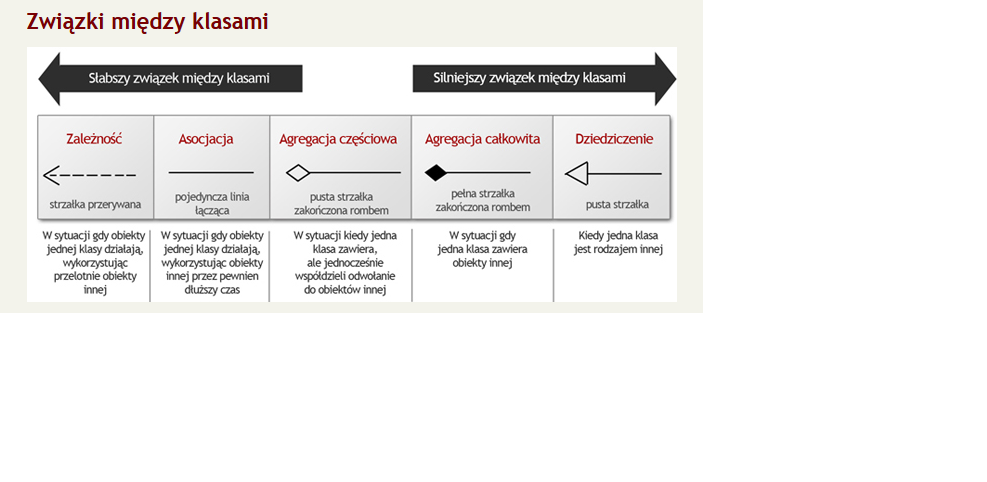
\includegraphics[width=.9\linewidth]{./zwiazki_UML.png}
\end{center}
\begin{center}

\includegraphics[width=.9\linewidth]{./uml.png}
\end{center}
\subsubsection{visibility (widocznosc)}
\label{sec:orgd79f67e}
\begin{itemize}
\item \texttt{+public}
\item \texttt{-private}
\item \texttt{\#protected}
\item \texttt{\textasciitilde{}package}
\end{itemize}
\subsubsection{asocjacja}
\label{sec:org3a87cb1}
\begin{itemize}
\item asocjacja - linia
\item asocjacja kierunkowa - linia z strzalka
\item agregacja(has-a) - pusty romb
\item kompozycja (agregacja mocna/calkowita) - zamalowany romb
\end{itemize}

\begin{enumerate}
\item kompozycja vs agregacja
\label{sec:org87328f8}
przy kompozycji jezeli niszczymy rodzica to dziecko tez ginie
\end{enumerate}
\subsubsection{dziedziczenie (generalizacja) is-a}
\label{sec:org83d04fc}
\subsubsection{implementacja (do intefejsow/abstract)}
\label{sec:orgb8d31d1}
\subsection{diagram sekwencji (sequence)}
\label{sec:org969cbeb}
czas od gory do dolu 
\subsection{diagram przypadkow uzycia (use case)}
\label{sec:org409ef42}
Graficzne przedstawienie przypadków użycia, aktorów oraz związków między nimi, występujących w danej dziedzinie przedmiotowej.

Diagram przypadków użycia w języku UML służy do modelowania funkcjonalności systemu. Tworzony jest zazwyczaj w początkowych fazach modelowania.

Diagram ten stanowi tylko przegląd możliwych działań w systemie, szczegóły ich przebiegu są modelowane za pomocą innych technik

Diagram przypadków użycia przedstawia usługi, które system świadczy aktorom, lecz bez wskazywania konkretnych rozwiązań technicznych.


\begin{itemize}
\item identyfikacja oraz dokumentacja wymagań,
\item umożliwiają analizę obszaru zastosowań, dziedziny przedmiotowej,
\item pozwalają na opracowanie projektu przyszłego systemu,
\item stanowią przystępną i zrozumiałą platformę współpracy i komunikacji twórców systemu, inwestorów i właścicieli,
\item są rodzajem umowy, kontraktu pomiędzy udziałowcami co do zakresu i funkcjonalności przyszłego systemu,
\item stanowią podstawę testowania funkcji systemu na dalszych etapach jego cyklu życia.
\end{itemize}

\subsubsection{asocjacja skierowana}
\label{sec:org6257254}
Asocjacja skierowana (ang. directed association) – asocjacja skierowana dziedziczy wszystkie cechy po asocjacji, lecz dodatkowo wskazuje kierunek nawigacji. Używana kiedy chcemy ukazać inicjatora interakcji (np. Aktor "Klient" jest inicjatorem przypadku użycia "Kup produkt").
\section{BPMN}
\label{sec:org9a493d7}
\subsection{zdarzenia}
\label{sec:org25a2e8a}
\begin{center}
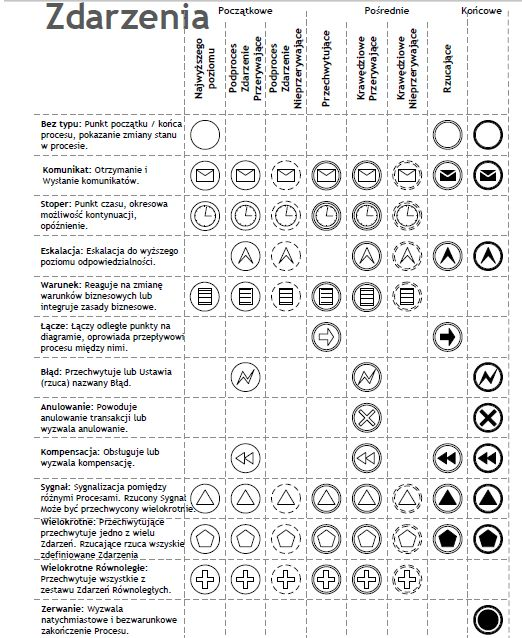
\includegraphics[width=.9\linewidth]{./zdarzenia.png}
\end{center}
\subsection{bramki}
\label{sec:orge5f2d61}
\begin{center}
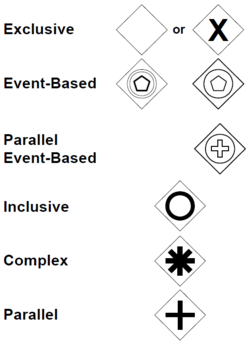
\includegraphics[width=.9\linewidth]{./bpmngate.png}
\end{center}
\section{wzorce kreacyjne}
\label{sec:org0d07884}
\subsection{singleton}
\label{sec:org2e3b3f1}
\url{https://refactoring.guru/design-patterns/singleton}

\begin{center}
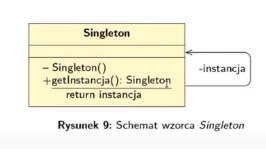
\includegraphics[width=.9\linewidth]{./singleton.png}
\end{center}
\begin{itemize}
\item zagwaratowac ze jest jeden obiekt tego typu (np. konfiguracja/stan globalny)
\item gdy w twoim programie ma prawo istnieć wyłącznie jeden ogólnodostępny obiekt danej klasy. Przykładem może być połączenie z bazą danych, którego używa wiele fragmentów programu.
\item gdy potrzebujesz ściślejszej kontroli nad zmiennymi globalnymi.
\end{itemize}
\subsubsection{implementacja}
\label{sec:orgc98e028}
\begin{verbatim}

class singleton {

private static singleton; //nasz obiekt
public static singleton getSingleton() //statyczna publiczna funkcja do otrzymywania tego stanu
{
	if(instancja==null)
		instancja = new Singleton();

	return singleton;
}
};

\end{verbatim}
\subsection{metoda wytworcza (factory method)}
\label{sec:orgf2542d1}
\begin{center}
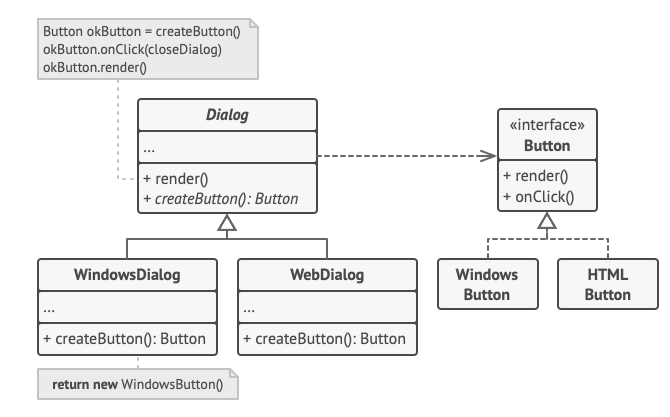
\includegraphics[width=.9\linewidth]{./factory.png}
\end{center}
\begin{itemize}
\item udostępnia interfejs do tworzenia obiektów w ramach klasy bazowej, ale pozwala podklasom zmieniać typ tworzonych obiektów.
\item Stosuj Metodę Wytwórczą gdy nie wiesz z góry jakie typy obiektów pojawią się w twoim programie i jakie będą między nimi zależności.
\item Metody Wytwórczej gdy zamierzasz pozwolić użytkującym twą bibliotekę lub framework rozbudowywać jej wewnętrzne komponenty.
\item gdy chcesz oszczędniej wykorzystać zasoby systemowe poprzez ponowne wykorzystanie już istniejących obiektów, zamiast odbudowywać je raz za razem.
\end{itemize}

Metoda Wytwórcza oddziela kod konstruujący produkty od kodu który faktycznie z tych produktów korzysta. Dlatego też łatwiej jest rozszerzać kod konstruujący produkty bez konieczności ingerencji w resztę kodu.
\subsection{fabryka abstrakcyjna (abstract factory)}
\label{sec:org6d99823}
\begin{center}
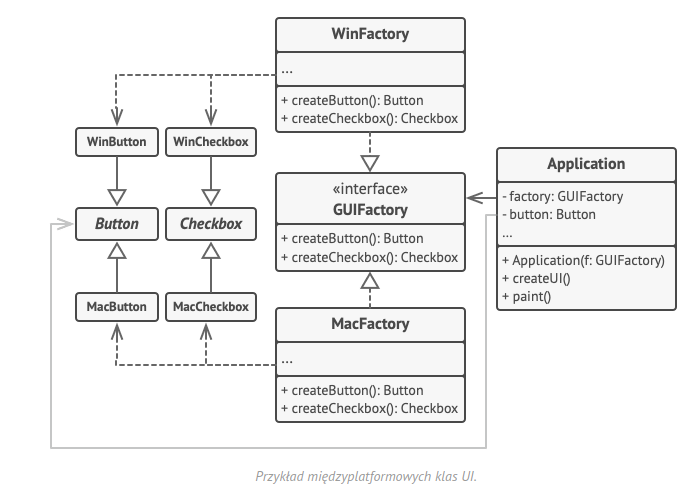
\includegraphics[width=.9\linewidth]{./abstractfactory.png}
\end{center}
\begin{itemize}
\item który pozwala tworzyć rodziny spokrewnionych ze sobą obiektów bez określania ich konkretnych klas.
\item gdy twój kod ma działać na produktach z różnych rodzin, ale jednocześnie nie chcesz, aby ściśle zależał od konkretnych klas produktów. Mogą one bowiem być nieznane na wcześniejszym etapie tworzenia programu, albo chcesz umożliwić przyszłą rozszerzalność aplikacji.
\item dostarcza ci interfejs służący tworzeniu obiektów z różnych klas danej rodziny produktów. O ile twój kod będzie kreował obiekty za pośrednictwem tego interfejsu — nie musisz się martwić stworzeniem produktu w niezgodnym z innymi wariancie.
\end{itemize}
\subsection{budowniczy (builder)}
\label{sec:orgd1de1da}
\begin{itemize}
\item \textbf{SKLADANIE OBIEKTU Z MALYCH CZESCI} np fabryka pizzy, konstruujesz ciasto, dodatki i sos
\item gdy potrzebujesz możliwości tworzenia różnych reprezentacji jakiegoś produktu (na przykład, domy z kamienia i domy z drewna).
\item Stosuj ten wzorzec do konstruowania drzew Kompozytowych lub innych złożonych obiektów.
\item Stosuj wzorzec Budowniczy, aby pozbyć się “teleskopowych konstruktorów”.
\end{itemize}
\begin{verbatim}
Pizza(int size) {  }
Pizza(int size, boolean cheese) {  }
Pizza(int size, boolean cheese, boolean pepperoni) {  }
\end{verbatim}

\subsubsection{problem}
\label{sec:orgc353007}
Wyobraź sobie jakiś skomplikowany obiekt, którego inicjalizacja jest pracochłonnym, wieloetapowym procesem obejmującym wiele pól i obiektów zagnieżdżonych. Taki kod inicjalizacyjny jest często wrzucany do wielgachnego konstruktora, przyjmującego mnóstwo parametrów. Albo jeszcze gorzej: kod taki rozrzucono po całym kodzie klienckim.
\subsection{prototyp}
\label{sec:org0c6b3a1}
\begin{itemize}
\item który umożliwia kopiowanie już istniejących obiektów bez tworzenia zależności pomiędzy twoim kodem, a klasami obiektów.
\item deleguje proces klonowania samym obiektom, które mają być sklonowane. We wzorcu tym deklarowany jest wspólny interfejs dla wszystkich obiektów wspierających funkcjonalność klonowania.
\end{itemize}

\section{wzorce behawioralne}
\label{sec:org0b11576}
\subsection{Obserwator (observer)}
\label{sec:orgd763a6f}
\begin{center}
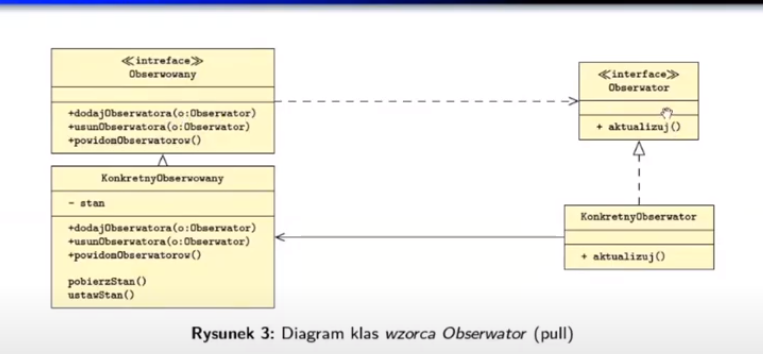
\includegraphics[width=.9\linewidth]{./obserwator.png}
\end{center}
\begin{itemize}
\item okresla zaleznosc jeden do wiele miedzy obiektami
\item gdy jeden obiekt zmienia stan wszystkie obiekty od niego zalezne sa o tym automatycznie powiadamiane i same sie uaktualniaja (np. w kalkulatorze mamy 3 klasy wypisywania ktore maja w sobie string do wypisywania, kiedy wprowadzamy nowe dzialanie wszyskie dostaja powiadomienie i sie  updatuja)
\item wydaje mi sie ze realizowany w grach -> bo trzeba updatowac stan obiektow a one musza znac stan innych
\item gdy zmiany stanu jednego obiektu mogą wymagać zmiany w innych obiektach, a konkretny zestaw obiektów nie jest zawczasu znany lub ulega zmianom dynamicznie
\item gdy jakieś obiekty w twojej aplikacji muszą obserwować inne, ale tylko przez jakiś czas lub w niektórych przypadkach.
\end{itemize}
\subsubsection{kontekst}
\label{sec:org77c5e77}
zmiana stanu jednego obiektu wymaga zmiany innych i nie wiadomo, ile obiektow trzeba zmienic
\subsubsection{problem}
\label{sec:org87a1217}
obiekt powinien byc w stanie powiadamiac inne obiekty, nie przyjmujac zadnych zalozen co do tego, co te obiekty reprezentuja - wynikiem sa luzniejsze powiazania miedzy obiektami
\subsubsection{implementacja}
\label{sec:org583e97d}
\url{https://refactoring.guru/design-patterns/observer}
zagwarantowanie ze przed rozeslaniem powiadomienia stan obserwowanergo jest wewnetrznie spojny


model push (obserwowany wysyla wszystkie informacje same)
model pull (obserwowany wysyla POWIADOMIENIE a kazdy inny pyta sie to czego potrzebuje z jakiejs zmiany)
\subsection{Stan (state)}
\label{sec:org94a3035}
\url{https://refactoring.guru/design-patterns/state}
\begin{itemize}
\item umozliwia obiektowi zmiane zachowania, gdy zmienia sie jego stan wewnetrzny (np. ktos zmienia typ konta bankowego)
\item gdy masz do czynienia z obiektem którego zachowanie jest zależne od jego stanu, liczba możliwych stanów jest wielka, a kod specyficzny dla danego stanu często ulega zmianom.
\item gdy masz klasę zaśmieconą rozbudowanymi instrukcjami warunkowymi zmieniającymi zachowanie klasy zależnie od wartości jej pól.
\item pomaga poradzić sobie z dużą ilością kodu który się powtarza w wielu stanach i przejściach między stanami automatu skończonego, bazującego na instrukcjach warunkowych.
\end{itemize}
\subsubsection{kontekst}
\label{sec:orga45e69e}
\begin{itemize}
\item zachowanie obiektu zalezy od jego stanu, a obiekt ten musi zmieniac swoje zachowanie w czasie wykonywania programu w zaleznosci od stanu
\item operacje zawieraja duze, wieloczesciowe instrukcje warunkowe ktore zaleza od stanu obiektu - wzorzec State przenosi kazde rozgalezienie do specjalnej klasy z inna implementacja np. pobierz podatek
\end{itemize}
\subsubsection{problem}
\label{sec:orgf3d4119}
chemy umozliwic obiektowi zmiane zachowania w momencie zmiany wewnetrzengo stanu obiektu hermetyzujac stan w postaci klasy
\subsubsection{implementacja}
\label{sec:org4cb1531}
\begin{center}
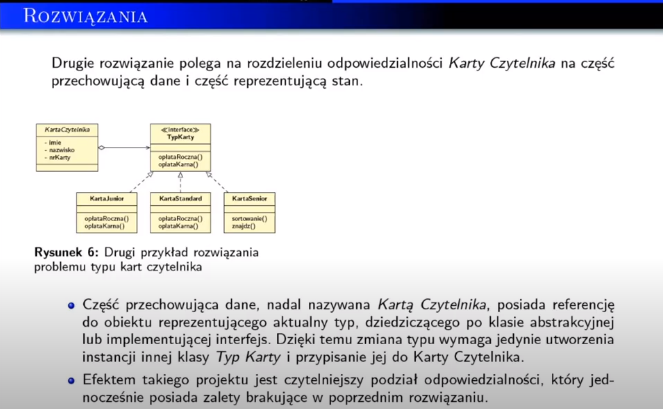
\includegraphics[width=.9\linewidth]{./stan.png}
\end{center}
\subsection{strategia (strategy)}
\label{sec:org6bb926f}
\begin{center}
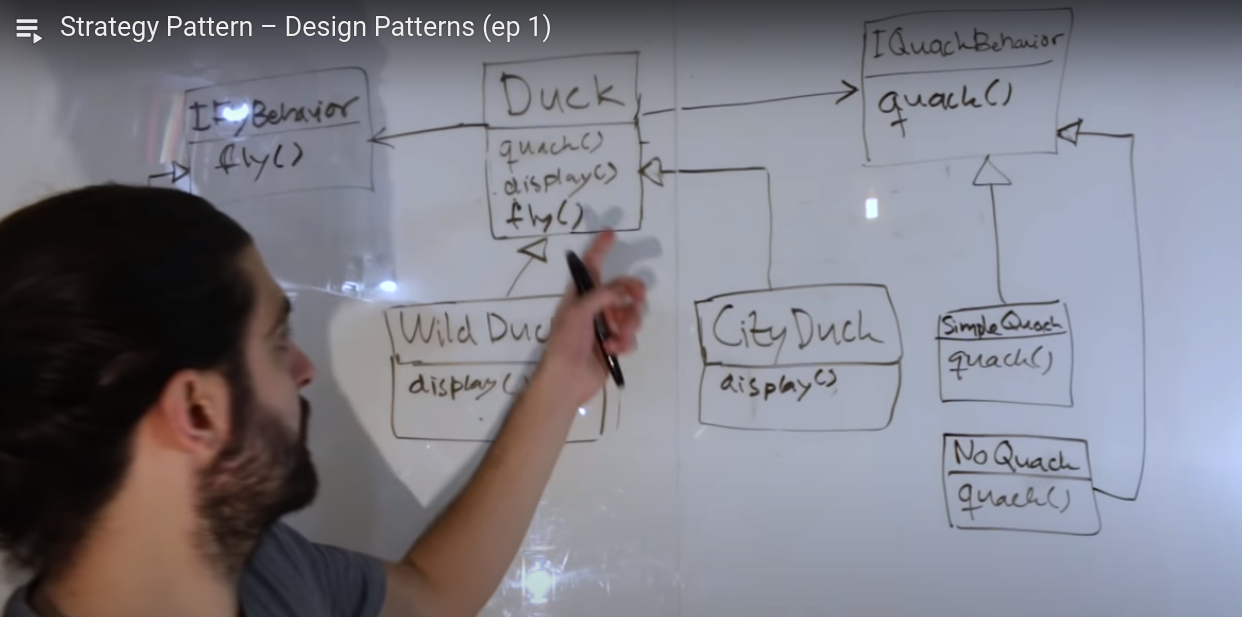
\includegraphics[width=.9\linewidth]{./strategy.png}
\end{center}

\url{https://refactoring.guru/design-patterns/strategy}
\begin{itemize}
\item roznica w implementacji ze stanem
\item w stanie klient nie widzi z kim dziala
\item w strategi klient zna wewnetrzna strukture - wie kto uzywa
\item pomaga poradzić sobie z dużą ilością kodu który się powtarza w wielu stanach i przejściach między stanami automatu skończonego, bazującego na instrukcjach warunkowych.
\item gdy masz w programie wiele podobnych klas, różniących się jedynie sposobem wykonywania jakichś zadań.
\item odizolować logikę biznesową klasy od szczegółów implementacyjnych algorytmów, które nie są istotne w kontekście tej logiki.
\item gdy twoja klasa zawiera duży operator warunkowy, którego zadaniem jest wybór odpowiedniego wariantu tego samego algorytmu.
\end{itemize}
\subsection{iterator}
\label{sec:org92de67b}
\begin{itemize}
\item hermetyzacja iteracji
\item gdy kolekcja z którą masz do czynienia posiada skomplikowaną strukturę, ale zależy ci na ukryciu jej przed klientem (dla wygody, lub dla bezpieczeństwa).
\item w celu redukcji duplikowania kodu przeglądania elementów zbiorów na przestrzeni całego programu.
\item gdy chcesz, aby twój kod był w stanie przeglądać elementy różnych struktur danych, lub gdy nie znasz z góry szczegółów ich struktury.
\item abstrakcja dla skomplikowanych struktur danych np. drzewo lista
\end{itemize}
\begin{verbatim}
Iterator iterator = menuCostam.utworzIterator();
while (iterator.hasNext())
{
 pozycjaMenu pozycja = iterator.next();
}
\end{verbatim}

\subsection{mediator}
\label{sec:org1c845bd}
pozwalający zredukować chaos zależności pomiędzy obiektami. Wzorzec ten ogranicza bezpośrednią komunikację pomiędzy obiektami i zmusza je do współpracy wyłącznie za pośrednictwem obiektu mediatora

\begin{itemize}
\item pozwalający zredukować chaos zależności pomiędzy obiektami. Wzorzec ten ogranicza bezpośrednią komunikację pomiędzy obiektami i zmusza je do współpracy wyłącznie za pośrednictwem obiektu mediatora
\item gdy nie możesz ponownie użyć jakiegoś komponentu w innym programie, z powodu zbytniej jego zależności od innych komponentow
\end{itemize}
gdy zauważysz, że tworzysz mnóstwo podklas komponentu tylko aby móc ponownie użyć jakieś zachowanie w innych kontekstach.
\subsection{Metoda szablonowa (template method)}
\label{sec:org0201f09}
\url{./template}
definiujący szkielet algorytmu w klasie bazowej, ale pozwalający podklasom nadpisać pewne etapy tego algorytmu bez konieczności zmiany jego struktury.
\begin{itemize}
\item gdy chcesz pozwolić klientom na rozszerzanie niektórych tylko etapów algorytmu, ale nie całego, ani też jego struktury.
\item gdy masz wiele klas zawierających niemal identyczne algorytmy różniące się jedynie szczegółami.  W takiej sytuacji bowiem konieczność modyfikacji algorytmu skutkuje koniecznością modyfikacji wszystkich klas.
\end{itemize}
\subsection{Odwiedzajacy (visitor)}
\label{sec:orgc30128b}
\begin{itemize}
\item gdy istnieje potrzeba wykonywania jakiegoś działania na wszystkich elementach złożonej struktury obiektów (jak drzewo obiektów).
\item pozwala uprzątnąć logikę biznesową czynności pomocniczych.
\item Warto stosować ten wzorzec gdy jakieś zachowanie ma sens tylko w kontekście niektórych klas wchodzących w skład hierarchii klas, ale nie wszystkich.
\end{itemize}
\subsection{polecenie (command)}
\label{sec:org0a5286c}
który zmienia żądanie w samodzielny obiekt zawierający wszystkie informacje o tym żądaniu. Taka transformacja pozwala na parametryzowanie metod przy użyciu różnych żądań. Oprócz tego umożliwia opóźnianie lub kolejkowanie wykonywania żądań oraz pozwala na cofanie operacji.
\begin{itemize}
\item gdy chcesz parametryzować obiekty za pomocą działań.
\item pozwala układać kolejki zadań, ustalać harmonogram ich wykonania bądź uruchamiać je zdalnie.
\end{itemize}
\section{wzorce strukturalne}
\label{sec:org722227f}
\subsection{kompozyt (composite)}
\label{sec:org4749293}
\begin{center}
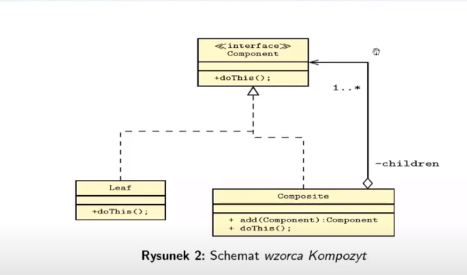
\includegraphics[width=.9\linewidth]{./kompozyt.png}
\end{center}
TLDR: Drzewko w ktorym lisc zawiera siebie + liste dzieci

\begin{itemize}
\item zadaniem jest laczenie obiektow w struktura tak, ze reprezentuja hierarchie czesci-calosci, unifikujac dostep do kolekcji jak i pojedynczego obiektu.
\item umozliwa to klientom jednolite traktowanie pojedynczych obiektow i rowniez ich kompozycji
\item Stosuj wzorzec Kompozyt gdy musisz zaimplementować drzewiastą strukturę obiektów.
\item Stosuj ten wzorzec gdy chcesz, aby kod kliencki traktował zarówno proste, jak i złożone elementy jednakowo.
\end{itemize}

\subsubsection{kontekst}
\label{sec:orgbe396b3}
chcemy przedstawic hierarchie obiektow czesc-calosc Hierarchia obiektow ma wspolna klase bazowa (abstrakcyjną)
\subsubsection{problem}
\label{sec:orgb7d004d}
chcemy, aby klienci mogli ignorowac roznice miedzy zlozeniami obiektow a pojedynczymi obiektami - klienci beda wtedy jednakowo traktowac wszyskie obiekty wystepujace w strukturze
\subsection{dekorator (decorator)}
\label{sec:orga3598d3}
\begin{center}
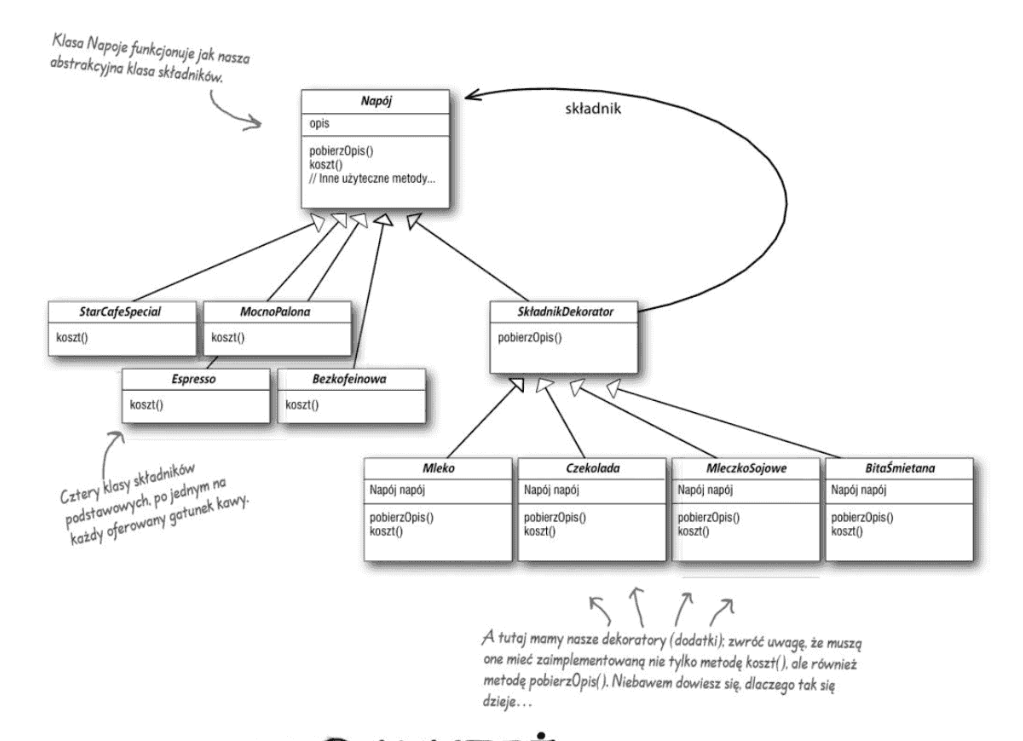
\includegraphics[width=.9\linewidth]{./dekorator.png}
\end{center}

pozwalający dodawać nowe obowiązki obiektom poprzez umieszczanie tych obiektów w specjalnych obiektach opakowujących, które zawierają odpowiednie zachowania.
\begin{itemize}
\item dodawanie dodatkowej funkcjonalnosci do obiektow
\item gdy chcesz przypisywać dodatkowe obowiązki obiektom w trakcie działania programu, bez psucia kodu, który z tych obiektów korzysta.
\item gdy rozszerzenie zakresu obowiązków obiektu za pomocą dziedziczenia byłoby niepraktyczne, lub niemożliwe.
\end{itemize}
\subsection{pelnomocnik (proxy)}
\label{sec:orgc48ded3}
pozwalający stworzyć obiekt zastępczy w miejsce innego obiektu. Pełnomocnik nadzoruje dostęp do pierwotnego obiektu, pozwalając na wykonanie jakiejś czynności przed lub po przekazaniu do niego żądania
\begin{itemize}
\item Leniwa inicjalizacja (wirtualny pełnomocnik). Gdy masz do czynienia z zasobożernym obiektem usługi, którego potrzebujesz jedynie co jakiś czas.
\item Kontrola dostępu (pełnomocnik ochronny). Przydatne, gdy chcesz pozwolić tylko niektórym klientom na korzystanie z obiektu usługi. Na przykład, gdy usługi stanowią kluczową część systemu operacyjnego, a klienci to różne uruchamiane aplikacje (również te szkodliwe).
\item Lokalne uruchamianie zdalnej usługi (pełnomocnik zdalny). Użyteczne, gdy obiekt udostępniający usługę znajduje się na zdalnym serwerze.
\item Prowadzenie dziennika żądań (pełnomocnik prowadzący dziennik). Pozwala prowadzić rejestr żądań przesyłanych do obiektu usługi.
\item Przechowywanie w pamięci podręcznej wyników działań (pełnomocnik z pamięcią podręczną). Pozwala przechować wyniki przekazywanych żądań i zarządzać cyklem życia pamięci podręcznej. Szczególnie ważne przy dużych wielkościach danych wynikowych.
\item Sprytne referencje. Można likwidować zasobożerny obiekt, gdy nie ma klientów którzy go potrzebują.
\end{itemize}
\subsection{fasada (facade)}
\label{sec:org9fedd42}
\begin{center}
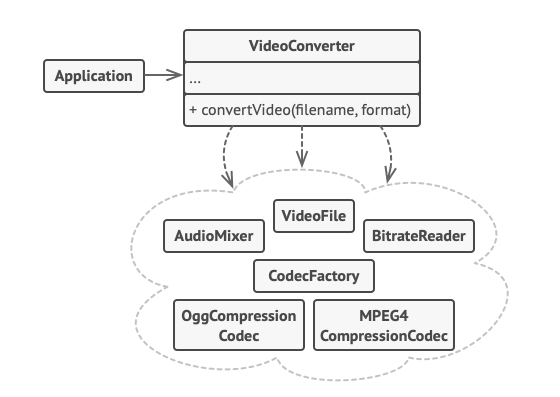
\includegraphics[width=.9\linewidth]{./facade.png}
\end{center}
który wyposaża bibliotekę, framework lub inny złożony zestaw klas w uproszczony interfejs.
\begin{itemize}
\item taki wrapper na wiele rzeczy
\item gdy potrzebujesz ograniczonego, ale łatwego w użyciu interfejsu do złożonego podsystemu.
\item gdy chcesz ustrukturyzować podsystem w warstwy.
\end{itemize}

\subsection{most (bridge)}
\label{sec:orgd99d2f1}
\begin{center}
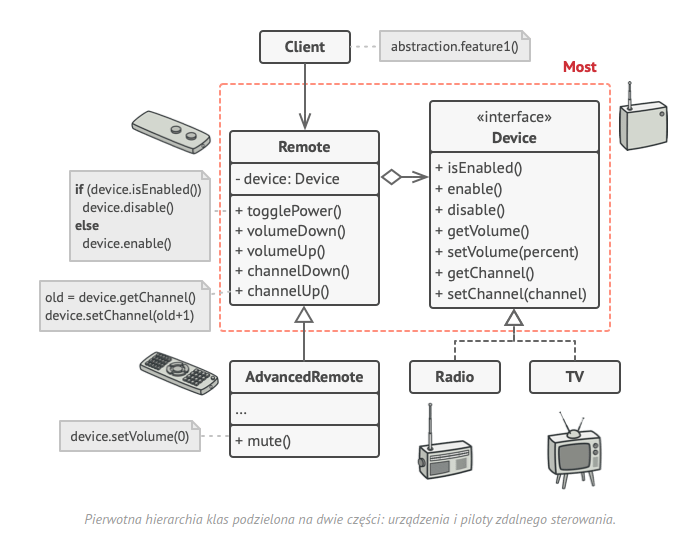
\includegraphics[width=.9\linewidth]{./bridge.png}
\end{center}
pozwalającym na rozdzielenie dużej klasy lub zestawu spokrewnionych klas na dwie hierarchie — abstrakcję oraz implementację. Nad obiema można wówczas pracować niezależnie.
\begin{itemize}
\item gdy chcesz rozdzielić i przeorganizować monolityczną klasę posiadającą wiele wariantów takiej samej funkcjonalności (na przykład, jeśli klasa ma współpracować z wieloma serwerami bazodanowymi).
\item gdy chcesz rozszerzyć klasę na kilku niezależnych płaszczyznach.
\item pozwala spełnić wymóg możliwości wyboru implementacji w trakcie działania programu.
\end{itemize}
\subsection{adapter}
\label{sec:org7cb5e5c}
\begin{center}
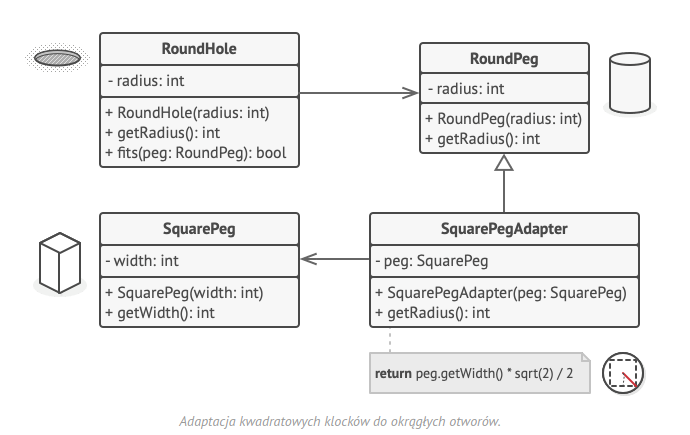
\includegraphics[width=.9\linewidth]{./adapter.png}
\end{center}
pozwalającym na współdziałanie ze sobą obiektów o niekompatybilnych interfejsach.
\begin{itemize}
\item gdy chcesz wykorzystać jakąś istniejącą klasę, ale jej interfejs nie jest kompatybilny z resztą twojego programu.
\item gdy chcesz wykorzystać ponownie wiele istniejących podklas którym brakuje jakiejś wspólnej funkcjonalności, niedającej się dodać do ich nadklasy.
\end{itemize}
\subsection{pylek (cache, flyweight)}
\label{sec:org3bd0284}
\begin{center}
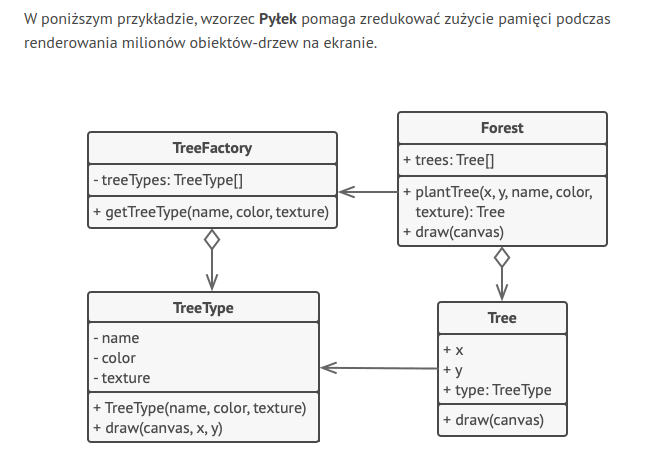
\includegraphics[width=.9\linewidth]{./cache.png}
\end{center}
pozwalającym zmieścić więcej obiektów w danej przestrzeni pamięci RAM poprzez współdzielenie części opisu ich stanów.
\begin{itemize}
\item gdy twój program musi pracować z wielką ilością obiektów, które ledwo mieszczą się w dostępnej pamięci RAM.
\end{itemize}
\section{pytania zamkniete}
\label{sec:orgdeedf5c}
\subsection{zaznacz glownie rodzaje procesow biznesowych}
\label{sec:org1bf7bc3}
procesy operacyjne, zarzadzcze i pomocnicze
\subsection{stosujac wzorzec <BLANK> gdy nie wiesz z gory jakie typy obiektow pojawiaja sie jakie twoim programie miedzy nimi zaleznosci}
\label{sec:org678d60a}
\textbf{factory method}
\subsection{stosujac wzorzec <BLANK> gdy istnieje potrzeba wykonywanie jakiego dzialania na elementach zlozonej strukty obiektow (jak drzewo obiektow)}
\label{sec:org8428b1c}
iterator
\subsection{stosuj wzorzec <BLANK> gdy musisz zaimplementowac drzewiasta strukture obiektow}
\label{sec:org7b25ba6}
\textbf{composite}
\subsection{korzystajac z wzorcza <BLANK> gdy chcesz oszczedniej wykorzystac zasoby systemowe poprzez ponownie wykorzystanie juz istniejacych obiektow zamiast odbudowywyac je raz za razem}
\label{sec:org2bf8ebe}
\textbf{factory method}
\subsection{stosuj wzorczec <BLANK> gdy chcesz przyjmowac dodatkow dodatkowe obowiazki obiektom w trajcie dziala programu, bez pisania \ldots{} ktory z tych obiektow korzysta}
\label{sec:orgb48513b}
\textbf{DEKORATOR} 
\subsection{stosowanie wzorcza <BLANK> pozwala uprzatnac logike biznesowa czynnosci pomocniczych}
\label{sec:org91d87eb}
\textbf{visitor}
\subsection{<BLANK> pozwala odizolowac logike biznesowa klasy od szczegolow implementacyjnych algorytmow, ktore nie sa istotne w kontekscie tej logiki}
\label{sec:org2d0db39}
\textbf{strategy} 
\subsection{stosuj wzorzec <BLANK> gdy chcesz aby kod klienci traktowal zarowno proste, jak i zlozone elementy jednakowo}
\label{sec:org630e998}
\textbf{composite}
\subsection{stosuj wzorzec <BLANK> gdy istnieje potrzeba wykonania jakiegos na dzialania na wszystkich elementacj zlozonej struktury obiektow (jak drzewo obiektow)}
\label{sec:org477b1b3}
\textbf{vistor}
\subsection{korzystaj z wzorcza <BLANK> gdy zamierzasz pozwolic uzytkujacym twa biblioteke lub framework rozbudowywac jej wewnetrzne komponenty}
\label{sec:orgd7ce90d}
\textbf{factory method}

\subsection{ktore stwierdzenia sa prawdziwy, gdy aktor A uogulnia aktora B}
\label{sec:orgb8de459}
\begin{itemize}
\item B moze komunikowac sie z tymi samymi przypadkami uzycia co A
\item B dziedziczy wszystkie zwiazki A
\end{itemize}
\subsection{ktore z ponizszych stwierdzen charaktyryzuja przypadki uzycia}
\label{sec:org0392868}
\begin{itemize}
\item przypadki uzycia posuja procedyury stosowane w systemie
\item ???przypadki uzycia posuja funkcjonalnosc lub zachowanie oczekiwane od opracowanego systemu???
\end{itemize}
\subsection{wybierz zdania prawdziwe okreslajace pojecie \textbf{bledu logicznego} w oprogramowaniu}
\label{sec:orgb2d6a5e}
\begin{itemize}
\item wiekszosc wysilkow, podzas testowania programu, koncentruje sie na ich znajdowaniu
\item blad  logiczny powstaje, gdy zewnetrzne zdarzenie lub nie wykryt blad skladni zmusza proces do zatrzymania swojego dzialania
\end{itemize}
\subsection{Proces określania wymagań dla systemu informatycznego można podzielić na następujące fazy}
\label{sec:orgc976b64}
\begin{itemize}
\item Faza ustalania wymagań
\item Faza specyfikacji wymagań
\item Faza atestacji wymagań
\end{itemize}
\subsection{Kontekst systemu}
\label{sec:orgce83bdb}
\begin{itemize}
\item Jest częścią środowiska systemu, która jest istotna ze względu na definiowanie i zrozumienie wymagań dla tworzonego systemu.
\item Odseparowania kontekstu systemu od samego systemu oraz części rzeczywistości, która jest nieistotna dla tworzonego systemu. Definiowanie granic systemu polega na podjęciu decyzji, które aspekty będą implementowane w systemie, a które należą tylko do jego kontekstu.
\end{itemize}
\subsection{Zaznacz główne rodzaje procesów biznesowych}
\label{sec:org1992192}
\begin{itemize}
\item Procesy operacyjne
\item Procesy zarządzania
\item Procesy pomocnicze
\end{itemize}
\subsection{Strukturalne wzorce projektowe to}
\label{sec:orgc93d52c}
\begin{itemize}
\item Adapter
\item Most
\item Kompozyt
\item Dekorator
\item Fasada
\item Pyłek
\item Pełnomocnik
\end{itemize}
\subsection{Wybierz zdania prawdziwie określające pojęcie złożoności cyklometrycznej}
\label{sec:orgc4a8078}
\begin{itemize}
\item Złożoność cyklometryczna jest to liczba niezależnych ścieżek w programie
\item Złożoność cyklometryczna jest podstawową miarą złożoności dowolnego fragmentu kodu programu
\end{itemize}
\subsection{Które z poniższych stwierdzeń charakteryzuje przypadki użycia}
\label{sec:org773dd6e}
\begin{itemize}
\item Przypadki użycia opisują procedury stosowane w systemie
\item Przypadki użycia opisują opisują funkcjonalność lub zachowanie oczekiwane od opracowywanego systemu1
\end{itemize}
\subsection{Na poniższym rysunku podano diagram klas oposujacy kalendarz online ktore z ponizszych stwierdzen sa prawdziwe}
\label{sec:orgc837105}
\begin{center}
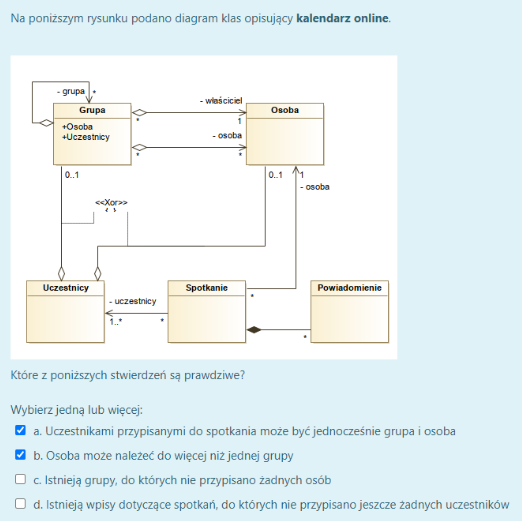
\includegraphics[width=.9\linewidth]{./zadanie1.png}
\end{center}
\begin{itemize}
\item osoba moze nalezec do wiecej niz jednej grupy
\item istnieja osoby, do ktorych nie rpzypisano zadnych osob
\end{itemize}
\subsection{Wybierz zdanie prawdziwe opisujace wzorzec strategia}
\label{sec:org2260921}
\begin{center}
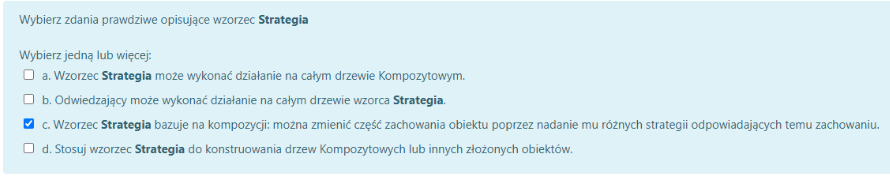
\includegraphics[width=.9\linewidth]{./zadanie2.png}
\end{center}
\begin{center}
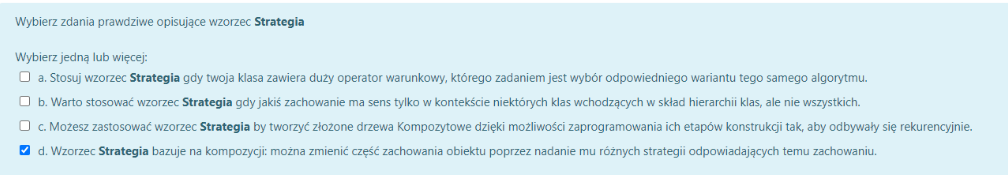
\includegraphics[width=.9\linewidth]{./zadanie10.png}
\end{center}
\begin{itemize}
\item wzorzec strategia bazuje na kompozycji: mozna zmienic czesc zachowania obiektu poprzed nadanie mu roznych strategi odpowiadajacych temu zachowaniu
\item wzorzec strategia bazuje na kompozycji: mozna zmienic czesc zachowania obiektu poprzez nadanie mu roznych strategi odpowiadajacych temu zachowaniu
\item stosuj wzorzec strategia gdy twoja klasa zawiera duzy operator warunkowy, ktorego zadaniem jest wybor odpoweidzniego wariantu tego samego algorytmu
\end{itemize}
\subsection{na ponizszym rysunku pokazano diagram sekwencji}
\label{sec:org56a25a5}
\begin{center}
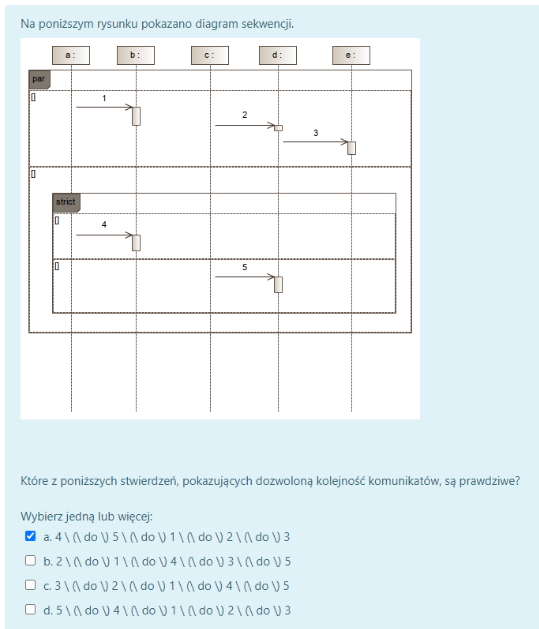
\includegraphics[width=.9\linewidth]{./zadanie3.png}
\end{center}
\begin{center}
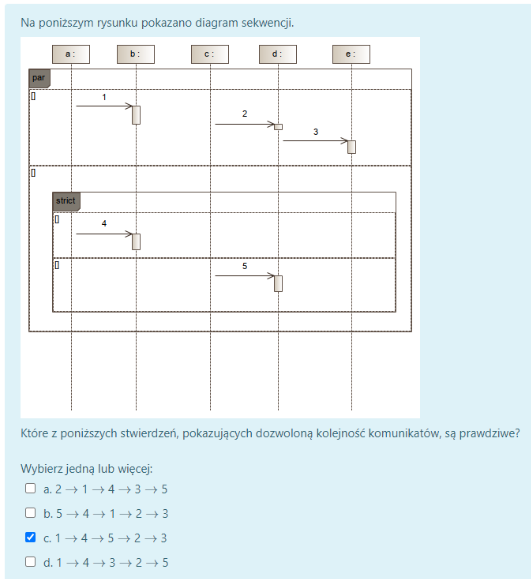
\includegraphics[width=.9\linewidth]{./zadanie12.png}
\end{center}
\subsection{wybierz zdania prawdziwe okreslajace testy jednostkowe}
\label{sec:org2402bca}
\begin{center}
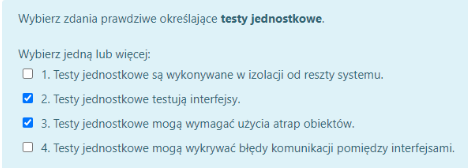
\includegraphics[width=.9\linewidth]{./zadanie4.png}
\end{center}
\begin{itemize}
\item testy jednostkowe moga wymagac uzycia atrap obiektow
\item testy jednostkowe sa wykonywane w izolacji od reszty systemu
\end{itemize}
\subsection{wybierz zdania prawdziwe okreslajace testy B  \(\beta\)}
\label{sec:org7d12b6f}
\begin{center}
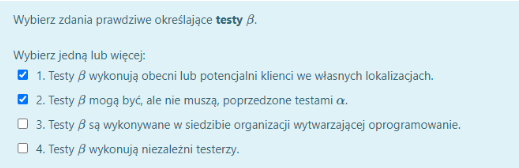
\includegraphics[width=.9\linewidth]{./zadanie5.png}
\end{center}
\begin{itemize}
\item testy \(\beta\) wykonuja obecni lub potencjalni klienci we wlasnych lokalizacjach
\item testy \(\beta\) moga byc, ale nie musza, poprzedzone testami \(\alpha\)
\end{itemize}
\subsection{na ponizszym rysunku podano diagram klas oposujacy kalendarz online}
\label{sec:orgd8212e3}
\begin{center}
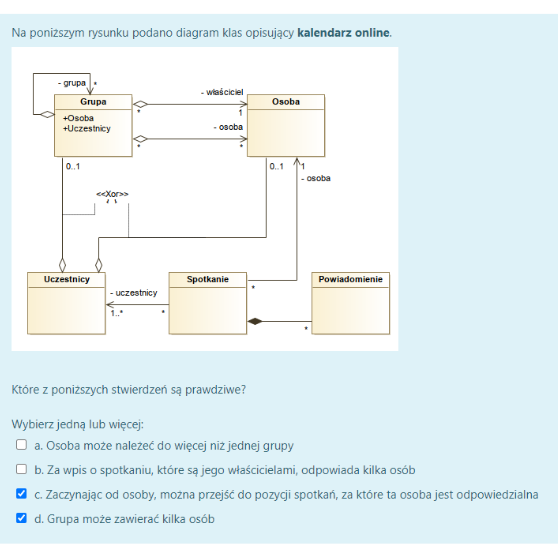
\includegraphics[width=.9\linewidth]{./zadanie6.png}
\end{center}
\begin{itemize}
\item grupa osob moze zawierac kilka osob
\item osoba moze nalezec dow iecej niz jednej grupy
\end{itemize}
\subsection{ktore z ponizszych stwierdzen dotyczacych pakietowego poziomu widocznosci sa poprawne}
\label{sec:org3510277}
\begin{center}
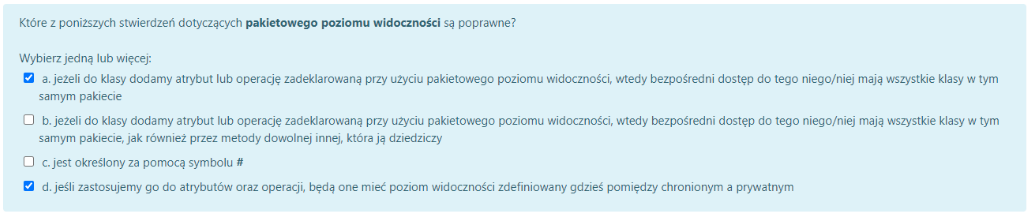
\includegraphics[width=.9\linewidth]{./zadanie7.png}
\end{center}
\begin{itemize}
\item jesli zastosujemy go do atrybutow oraz operacji, beda one miec poziom widocznosci zdefiniowany gdzies pomiedzy chronionym a prywatnym
\item jezeli do klasy dodamy atrybut lub operacje zadeklarowana przy uzyciu pakietowego poziomu widocznosci, tedy bezposredni dostep do tego niego/niej maja wszystki klasy w tym samym pakiecie
\end{itemize}
\subsection{wybierz zdania prawdziwe opisujace wzorzec kompozyt}
\label{sec:org315d9b8}
\begin{center}
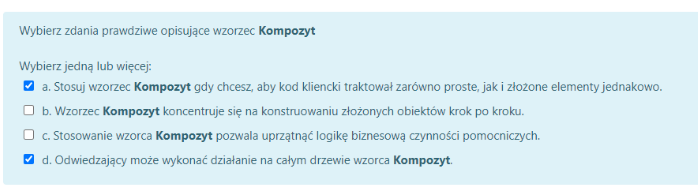
\includegraphics[width=.9\linewidth]{./zadanie8.png}
\end{center}
\begin{itemize}
\item stosuj wzorzec kompozyt gdy chcesz, aby kod kliencki traktowal zarowno proste, jak i zlozone elementy jednakowo
\item odwiedzajacy moze wyknac dzialanie na calym drzewie wzorca kompozyt
\end{itemize}
\subsection{agregacja \ldots{}}
\label{sec:org15eb521}
\begin{center}
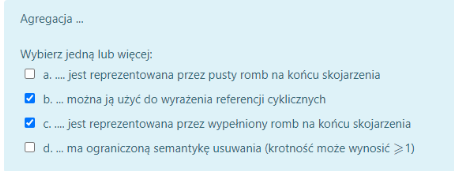
\includegraphics[width=.9\linewidth]{./zadanie9.png}
\end{center}
\begin{itemize}
\item jest reprezentowana przez pusty romb na koncu skojarzenia
\end{itemize}
\subsection{ktore stwierdzenia dotyczace ponizszego rysunku sa poprawne}
\label{sec:org668518b}
\begin{center}
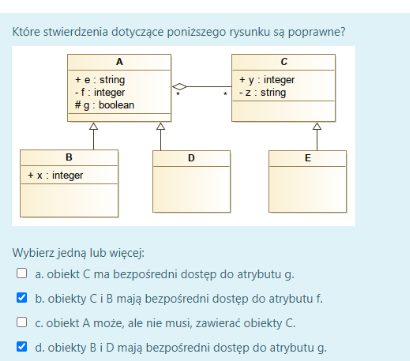
\includegraphics[width=.9\linewidth]{./zadanie11.png}
\end{center}

\subsection{wybierz zdania prawdziwe opisujace wzorzec budowniczy}
\label{sec:org217d2f7}
\begin{center}

\includegraphics[width=.9\linewidth]{./zadanie13.png}
\end{center}
\subsection{ktore z ponizszych pytan ma sens w identyfikacji aktorow na diagramie przypadkow uzycia}
\label{sec:orgaed0d69}
\begin{center}
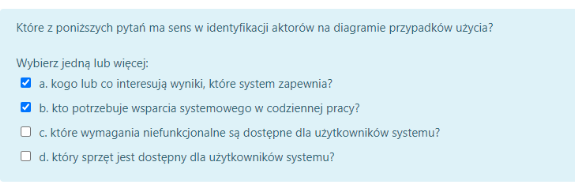
\includegraphics[width=.9\linewidth]{./zadanie14.png}
\end{center}
\subsection{ktore z ponizszych stwierdzen dotyczace komunkatow sa poprawne}
\label{sec:orgcb0fa35}
\begin{center}
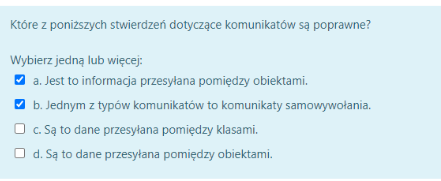
\includegraphics[width=.9\linewidth]{./zadanie15.png}
\end{center}
\subsection{ktore stwierdzenia dotyczace ponizszego rysunku sa poprawne}
\label{sec:orgb899610}
\begin{center}
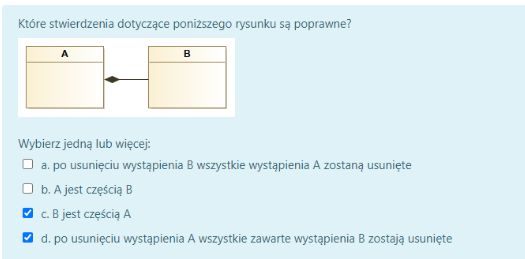
\includegraphics[width=.9\linewidth]{./zadanie16.png}
\end{center}
\section{pytania otwarte odpowiedz}
\label{sec:orgb31f6a3}
\subsection{kiedy nie nalezy stosowac dziedziczenia opisz przynajmniej dwa przypadki}
\label{sec:orga9a79f0}
\begin{itemize}
\item dont use inheritance for code reuse
\item kiedy dziedziczymy po klasie metody lub zmienne ktore dla naszego typu "powinny" byc nie zdefiniowane
\item brak pamieci
\end{itemize}
\subsection{opisac silnva agregacja}
\label{sec:org4a751f5}
to co agregacja + jak rodzic ginie to dziecko ginie
\section{pytania otwarte modelio}
\label{sec:org8bd7c86}
\subsection{system w ktorym pracownicy moga byc rowniez klientami, zaproponuj trzy rozwiazania opisujac i wady i zalety}
\label{sec:org89dbc39}
\subsection{zamodeluj podsystem obslugi klienta w sklepie internetowych Zacznij od opisu wymagan i procesow}
\label{sec:org405c672}
\end{document}
